\documentclass[journal]{IEEEtran}

\usepackage{lipsum}% http://ctan.org/pkg/lipsum
\usepackage{graphicx}% http://ctan.org/pkg/graphicx
% *** CITATION PACKAGES **
%
%\usepackage{cite}
% cite.sty was written by Donald Arseneau
% V1.6 and later of IEEEtran pre-defines the format of the cite.sty package
% \cite{} output to follow that of the IEEE. Loading the cite package will
% result in citation numbers being automatically sorted and properly
% "compressed/ranged". e.g., [1], [9], [2], [7], [5], [6] without using
% cite.sty will become [1], [2], [5]--[7], [9] using cite.sty. cite.sty's
% \cite will automatically add leading space, if needed. Use cite.sty's
% noadjust option (cite.sty V3.8 and later) if you want to turn this off
% such as if a citation ever needs to be enclosed in parenthesis.
% cite.sty is already installed on most LaTeX systems. Be sure and use
% version 5.0 (2009-03-20) and later if using hyperref.sty.
% The latest version can be obtained at:
% http://www.ctan.org/pkg/cite
% The documentation is contained in the cite.sty file itself.
% *** GRAPHICS RELATED PACKAGES ***
%
\ifCLASSINFOpdf
%\usepackage[pdftex]{graphicx}
  % declare the path(s) where your graphic files are
  % \graphicspath{{../pdf/}{../jpeg/}}
  % and their extensions so you won't have to specify these with
  % every instance of \includegraphics
  % \DeclareGraphicsExtensions{.pdf,.jpeg,.png}
\else
  % or other class option (dvipsone, dvipdf, if not using dvips). graphicx
  % will default to the driver specified in the system graphics.cfg if no
  % driver is specified.
  % \usepackage[dvips]{graphicx}
  % declare the path(s) where your graphic files are
  % \graphicspath{{../eps/}}
  % and their extensions so you won't have to specify these with
  % every instance of \includegraphics
  % \DeclareGraphicsExtensions{.eps}
\fi
% graphicx was written by David Carlisle and Sebastian Rahtz. It is
% required if you want graphics, photos, etc. graphicx.sty is already
% installed on most LaTeX systems. The latest version and documentation
% can be obtained at: 
% http://www.ctan.org/pkg/graphicx
% Another good source of documentation is "Using Imported Graphics in
% LaTeX2e" by Keith Reckdahl which can be found at:
% http://www.ctan.org/pkg/epslatex
%
% latex, and pdflatex in dvi mode, support graphics in encapsulated
% postscript (.eps) format. pdflatex in pdf mode supports graphics
% in .pdf, .jpeg, .png and .mps (metapost) formats. Users should ensure
% that all non-photo figures use a vector format (.eps, .pdf, .mps) and
% not a bitmapped formats (.jpeg, .png). The IEEE frowns on bitmapped formats
% which can result in "jaggedy"/blurry rendering of lines and letters as
% well as large increases in file sizes.
%
% You can find documentation about the pdfTeX application at:
% http://www.tug.org/applications/pdftex





% *** MATH PACKAGES ***
%
%\usepackage{amsmath}
% A popular package from the American Mathematical Society that provides
% many useful and powerful commands for dealing with mathematics.
%
% Note that the amsmath package sets \interdisplaylinepenalty to 10000
% thus preventing page breaks from occurring within multiline equations. Use:
%\interdisplaylinepenalty=2500
% after loading amsmath to restore such page breaks as IEEEtran.cls normally
% does. amsmath.sty is already installed on most LaTeX systems. The latest
% version and documentation can be obtained at:
% http://www.ctan.org/pkg/amsmath





% *** SPECIALIZED LIST PACKAGES ***
%
%\usepackage{algorithmic}
% algorithmic.sty was written by Peter Williams and Rogerio Brito.
% This package provides an algorithmic environment fo describing algorithms.
% You can use the algorithmic environment in-text or within a figure
% environment to provide for a floating algorithm. Do NOT use the algorithm
% floating environment provided by algorithm.sty (by the same authors) or
% algorithm2e.sty (by Christophe Fiorio) as the IEEE does not use dedicated
% algorithm float types and packages that provide these will not provide
% correct IEEE style captions. The latest version and documentation of
% algorithmic.sty can be obtained at:
% http://www.ctan.org/pkg/algorithms
% Also of interest may be the (relatively newer and more customizable)
% algorithmicx.sty package by Szasz Janos:
% http://www.ctan.org/pkg/algorithmicx




% *** ALIGNMENT PACKAGES ***
%
%\usepackage{array}
% Frank Mittelbach's and David Carlisle's array.sty patches and improves
% the standard LaTeX2e array and tabular environments to provide better
% appearance and additional user controls. As the default LaTeX2e table
% generation code is lacking to the point of almost being broken with
% respect to the quality of the end results, all users are strongly
% advised to use an enhanced (at the very least that provided by array.sty)
% set of table tools. array.sty is already installed on most systems. The
% latest version and documentation can be obtained at:
% http://www.ctan.org/pkg/array


% IEEEtran contains the IEEEeqnarray family of commands that can be used to
% generate multiline equations as well as matrices, tables, etc., of high
% quality.




% *** SUBFIGURE PACKAGES ***
%\ifCLASSOPTIONcompsoc
%  \usepackage[caption=false,font=normalsize,labelfont=sf,textfont=sf]{subfig}
%\else
%  \usepackage[caption=false,font=footnotesize]{subfig}
%\fi
% subfig.sty, written by Steven Douglas Cochran, is the modern replacement
% for subfigure.sty, the latter of which is no longer maintained and is
% incompatible with some LaTeX packages including fixltx2e. However,
% subfig.sty requires and automatically loads Axel Sommerfeldt's caption.sty
% which will override IEEEtran.cls' handling of captions and this will result
% in non-IEEE style figure/table captions. To prevent this problem, be sure
% and invoke subfig.sty's "caption=false" package option (available since
% subfig.sty version 1.3, 2005/06/28) as this is will preserve IEEEtran.cls
% handling of captions.
% Note that the Computer Society format requires a larger sans serif font
% than the serif footnote size font used in traditional IEEE formatting
% and thus the need to invoke different subfig.sty package options depending
% on whether compsoc mode has been enabled.
%
% The latest version and documentation of subfig.sty can be obtained at:
% http://www.ctan.org/pkg/subfig




% *** FLOAT PACKAGES ***
%
%\usepackage{fixltx2e}
% fixltx2e, the successor to the earlier fix2col.sty, was written by
% Frank Mittelbach and David Carlisle. This package corrects a few problems
% in the LaTeX2e kernel, the most notable of which is that in current
% LaTeX2e releases, the ordering of single and double column floats is not
% guaranteed to be preserved. Thus, an unpatched LaTeX2e can allow a
% single column figure to be placed prior to an earlier double column
% figure.
% Be aware that LaTeX2e kernels dated 2015 and later have fixltx2e.sty's
% corrections already built into the system in which case a warning will
% be issued if an attempt is made to load fixltx2e.sty as it is no longer
% needed.
% The latest version and documentation can be found at:
% http://www.ctan.org/pkg/fixltx2e


%\usepackage{stfloats}
% stfloats.sty was written by Sigitas Tolusis. This package gives LaTeX2e
% the ability to do double column floats at the bottom of the page as well
% as the top. (e.g., "\begin{figure*}[!b]" is not normally possible in
% LaTeX2e). It also provides a command:
%\fnbelowfloat
% to enable the placement of footnotes below bottom floats (the standard
% LaTeX2e kernel puts them above bottom floats). This is an invasive package
% which rewrites many portions of the LaTeX2e float routines. It may not work
% with other packages that modify the LaTeX2e float routines. The latest
% version and documentation can be obtained at:
% http://www.ctan.org/pkg/stfloats
% Do not use the stfloats baselinefloat ability as the IEEE does not allow
% \baselineskip to stretch. Authors submitting work to the IEEE should note
% that the IEEE rarely uses double column equations and that authors should try
% to avoid such use. Do not be tempted to use the cuted.sty or midfloat.sty
% packages (also by Sigitas Tolusis) as the IEEE does not format its papers in
% such ways.
% Do not attempt to use stfloats with fixltx2e as they are incompatible.
% Instead, use Morten Hogholm'a dblfloatfix which combines the features
% of both fixltx2e and stfloats:
%
% \usepackage{dblfloatfix}
% The latest version can be found at:
% http://www.ctan.org/pkg/dblfloatfix




%\ifCLASSOPTIONcaptionsoff
%  \usepackage[nomarkers]{endfloat}
% \let\MYoriglatexcaption\caption
% \renewcommand{\caption}[2][\relax]{\MYoriglatexcaption[#2]{#2}}
%\fi
% endfloat.sty was written by James Darrell McCauley, Jeff Goldberg and 
% Axel Sommerfeldt. This package may be useful when used in conjunction with 
% IEEEtran.cls'  captionsoff option. Some IEEE journals/societies require that
% submissions have lists of figures/tables at the end of the paper and that
% figures/tables without any captions are placed on a page by themselves at
% the end of the document. If needed, the draftcls IEEEtran class option or
% \CLASSINPUTbaselinestretch interface can be used to increase the line
% spacing as well. Be sure and use the nomarkers option of endfloat to
% prevent endfloat from "marking" where the figures would have been placed
% in the text. The two hack lines of code above are a slight modification of
% that suggested by in the endfloat docs (section 8.4.1) to ensure that
% the full captions always appear in the list of figures/tables - even if
% the user used the short optional argument of \caption[]{}.
% IEEE papers do not typically make use of \caption[]'s optional argument,
% so this should not be an issue. A similar trick can be used to disable
% captions of packages such as subfig.sty that lack options to turn off
% the subcaptions:
% For subfig.sty:
% \let\MYorigsubfloat\subfloat
% \renewcommand{\subfloat}[2][\relax]{\MYorigsubfloat[]{#2}}
% However, the above trick will not work if both optional arguments of
% the \subfloat command are used. Furthermore, there needs to be a
% description of each subfigure *somewhere* and endfloat does not add
% subfigure captions to its list of figures. Thus, the best approach is to
% avoid the use of subfigure captions (many IEEE journals avoid them anyway)
% and instead reference/explain all the subfigures within the main caption.
% The latest version of endfloat.sty and its documentation can obtained at:
% http://www.ctan.org/pkg/endfloat
%
% The IEEEtran \ifCLASSOPTIONcaptionsoff conditional can also be used
% later in the document, say, to conditionally put the References on a 
% page by themselves.




% *** PDF, URL AND HYPERLINK PACKAGES ***
%
\usepackage{url}
% url.sty was written by Donald Arseneau. It provides better support for
% handling and breaking URLs. url.sty is already installed on most LaTeX
% systems. The latest version and documentation can be obtained at:
% http://www.ctan.org/pkg/url
% Basically, \url{my_url_here}.




% *** Do not adjust lengths that control margins, column widths, etc. ***
% *** Do not use packages that alter fonts (such as pslatex).         ***
% There should be no need to do such things with IEEEtran.cls V1.6 and later.
% (Unless specifically asked to do so by the journal or conference you plan
% to submit to, of course. )


% correct bad hyphenation here
% \hyphenation{op-tical net-works semi-conduc-tor}


\begin{document}
%
% paper title
% Titles are generally capitalized except for words such as a, an, and, as,
% at, but, by, for, in, nor, of, on, or, the, to and up, which are usually
% not capitalized unless they are the first or last word of the title.
% Linebreaks \\ can be used within to get better formatting as desired.
% Do not put math or special symbols in the title.
\title{CS561 - Term Paper 1\\Big Data and Map Reduce}
%
%
% author names and IEEE memberships
% note positions of commas and nonbreaking spaces ( ~ ) LaTeX will not break
% a structure at a ~ so this keeps an author's name from being broken across
% two lines.
% use \thanks{} to gain access to the first footnote area
% a separate \thanks must be used for each paragraph as LaTeX2e's \thanks
% was not built to handle multiple paragraphs
%

\author{Abhishek,~\IEEEmembership{B15103,~B.Tech CSE 2015-19 Batch,~IIT Mandi}}


% The paper headers
\markboth{CS561 - Big Data and Map Reduce, Term Paper 1}{CS561 - Big Data and Map Reduce, Term Paper 1}

\maketitle

% As a general rule, do not put math, special symbols or citations
% in the abstract or keywords.
\begin{abstract}
\textit{Big Data} has become a huge trendy topic in the world of computing. Computation on big data, of course, is different than computation on a normal data, but the principles remain quite the same. Many technologies have come up for computing big data, but Hadoop Mapreduce has been one of the most popular technologies. In this term paper, we aim to analyze the current available technology for computation in big data, describe the Hadoop Mapreduce framework, and discuss some of the limitations of Mapreduce framework.
\end{abstract}

% Note that keywords are not normally used for peerreview papers.
\begin{IEEEkeywords}
Big Data, Apache Hadoop, Mapreduce framework
\end{IEEEkeywords}


% For peer review papers, you can put extra information on the cover
% page as needed:
% \ifCLASSOPTIONpeerreview
% \begin{center} \bfseries EDICS Category: 3-BBND \end{center}
% \fi
%
% For peerreview papers, this IEEEtran command inserts a page break and
% creates the second title. It will be ignored for other modes.
\IEEEpeerreviewmaketitle



\section{Introduction}
% The very first letter is a 2 line initial drop letter followed
% by the rest of the first word in caps.
% 
% form to use if the first word consists of a single letter:
% \IEEEPARstart{A}{demo} file is ....
% 
% form to use if you need the single drop letter followed by
% normal text (unknown if ever used by the IEEE):
% \IEEEPARstart{A}{}demo file is ....
% 
% Some journals put the first two words in caps:
% \IEEEPARstart{T}{his demo} file is ....
% 
% Here we have the typical use of a "T" for an initial drop letter
% and "HIS" in caps to complete the first word.
\IEEEPARstart{B}{ig} data refers to the data sets which are of the size beyond the current database technology. \cite{akerkar2013big} In this day and age of computing, the numbers on the size of data has increased very fast, and have gone outside the range of capability of a single computer. Although, it's size is huge, big data offers exciting aspects of computing as the sheer amount of information that can be extracted with this amount of data is very valuable for this day and age. Currently, all forms of huge amount of data can be classified as big data. Whether it be the data generated from online transactions, videos, YouTube, social media sites such as Twitter, Facebook, etc., sensors, blogs, search queries, health records all have the potential to be classified as big data. \cite{6567202}

It is estimated that almost 5 exabytes of data was created until the late 2003s. In comparison to that of today's data generation, such an amount of data can be generated in just a matter of two days. Intel has expected this amount to double every two years. \cite{IntelIT} A normal computer today has a capacity of at most couple of terabytes. If we need to store this amount of data on such computers, it would require about a million number of computers to store that amount of data. But it can be seen with such amount of data, that the amount of information that could be extracted from the big data is really golden. Big data analysis has helped achieving great leaps of progress in sectors such as healthcare, finance, research, etc.

With so many advantages, it does seem that big data is quite the way forward. But all is not so easy. Extraction of information from Big data poses a huge challenge some of which will be discussed in the next section. Many technologies have come up with solutions, but each have its own advantages and disadvantages. In the next section of this term paper, we analyze deeper into big data extraction and its challenges by the help of literature review. In the further sections we bring forward the technologies present today to deal with big data. Then we move forward to list some limitations of the popular Mapreduce framework, following a conclusion on the topic.

\section{Literature Review}

\subsection{Important Challenges posed by Big Data}
Big Data is characterized by its 3V features, namely, Volume, Velocity and Variety. The characteristics are explained as below -
	\begin{itemize}
    	\item \textbf{Velocity} - Extraction of information from big data has to be in a timely fashion. If the information is not able to be extracted in that time, then the data becomes useless in context of extractable information.
        \item \textbf{Volume} - As described earlier, the volume of big data has gone past the limit of capability of complex database systems. Hence, a new way of handling such a huge amount of data is required.
        \item \textbf{Variety} - Big data can be generated from almost every domain of life. But this data is not inherently structured or sorted as such. The data could vary in terms of representation, structure, etc. Hence, handling such type of data makes extraction of information from big data very difficult.
    \end{itemize}
\begin{figure}[!ht]
	\centering
    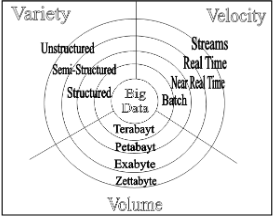
\includegraphics[scale=0.9]{Selection_038.png}
    \caption{The 3V's of big data. \cite{6567202}}
    \label{3v}
\end{figure}

\subsection{Data Collection}
Big data can be collected from various sources such as astronomy, medicine, engineering, research, business, etc. and can be analyzed and can also help in solving real problems. McKinsey Global Institute has found out the potential usage of big data in five main topics \cite{manyika2011big} :
	\begin{itemize}
		\item Healthcare
        \item Public sector
        \item Retail
        \item Manufacturing
        \item Personal location data
	\end{itemize}
 Though the data can be collected very easily, there comes a question of data privacy for users. This amount of data comes from the millions and billions of people who use the above five services, and the question of ethics prevail in this matter. As long as the data is being collected in consent of the people, data collection poses no great problem. \cite{ceravolo2018big}
% needed in second column of first page if using \IEEEpubid
%\IEEEpubidadjcol

\section{Current Technologies and Platforms}
There have been many technologies in the market for computing on big data. The technologies can be grouped mainly on the basis of scalability. Scalability is the capability of a system, network, or process to handle a growing amount of work, or its potential to be enlarged to accommodate that growth. \cite{Bondi} It can be viewed in terms of big data processing as the ability to cater huge amounts of data efficiently. Hence, the big data platforms can be classified into the following two types of scaling -
\begin{itemize}
\item Horizontal scaling - This type of scaling generally means adding more nodes over the distributed network to evenly distribute the load.
\item Vertical scaling - This type of scaling generally refers to adding of additional resources on a single computer.
\end{itemize}

Based on the two types of scaling, we will now see the platforms associated with it. \cite{Singh2014}

\subsection{Horizontal Scaling}

\subsubsection{\textbf{Peer-to-Peer Networks}}
Peer-to-Peer networks \cite{Singh2014} \cite{milojicic2002peer} \cite{steinmetz2005peer} is a network with a huge amount of computer nodes connected to it for computation purposes. It is an architecture which is decentralized as well as distributed as the nodes in the network (peers) serve as well as consume resources.

Message Passing Interface (MPI) is the communication medium used in Peer-to-Peer Networks. Each node can be vertically scaled and the the whole system or network could be easily horizontally scaled.

Although, Peer-to-Peer networks is quite simple, there is a huge bottleneck within the system which lies in the communication between different nodes. This could be solved by broadcasting the messages, but the accessing the accumulated data/results would be very expensive.

\subsubsection{\textbf{Apache Hadoop and MapReduce Framework}}
Apache Hadoop is an open source framework that is used for distributed processing on large data sets across a cluster of computers. The various components of a Hadoop Stack are shown in Figure \ref{stack}. The Hadoop platform contains the following two important components:
\begin{itemize}
\item \textbf{Distributed File System (HDFS)} \cite{borthakurhdfs} is a distributed file system that is used to store data across cluster of commodity machines while providing high availability and fault tolerance.
\item \textbf{Hadoop YARN} \cite{vavilapalli2013apache} is a resource management layer and schedules the jobs across the cluster.
\end{itemize}
\begin{figure}
\centering
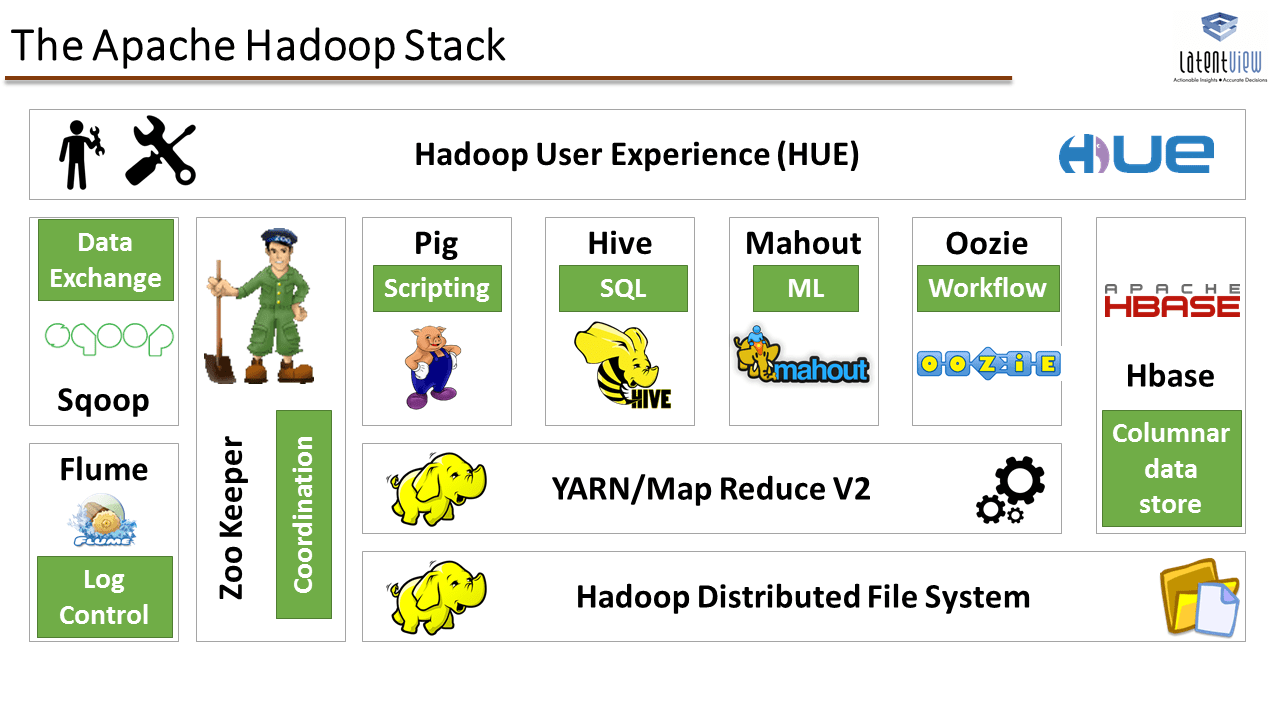
\includegraphics[width=0.45\textwidth]{hadoop-stack.png}
\caption{Apache Hadoop Stack \cite{spanish}}
\label{stack}
\end{figure}

Hadoop uses the \textbf{MapReduce} framework \cite{dean2008mapreduce} which was proposed by Dean and Ghemawat at Google, for its computation. MapReduce breaks the entire task into two parts, known as mappers and reducers. For a broad understanding, mappers read some input to generate some intermediate results, and these intermediate results are then passed to reducers, where the primary aggregation of results. Results are written to HDFS storage under the Hadoop stack. Mappers and reducers are distributed over the whole cluster of computing nodes. MapReduce can be divided into two stages \cite{bakshi2012considerations}
\begin{itemize}
\item \textit{Map Step} - The mapper's job is to simplify the input data into chunks of data which is stored on the local storage where the reducer can access it. \cite{6567202}  
\item \textit{Reduce Step} - This step takes the intermediate results and merge them in a parallel fashion to produce a set of output which is then stored on the HDFS. \cite{6567202}
\end{itemize}

The Hadoop technology was inspired by the BigTable technology which is Google's data storage system, Google File System and the MapReduce framework. Hadoop is a Java based framework and an open source platform. Although not designed for real-time systems and data streaming, Hadoop offers \cite{hadoop1} (also shown in Figure \ref{stack}) -
\begin{itemize}
\item \textit{HDFS} - A highly fault tolerant distributed file system that is responsible for storing data on the clusters.
\item \textit{MapReduce} - A powerful parallel programming technique for distributed processing on clusters.
\item \textit{HBase} - A scalable, distributed database for random read/write access.
\item \textit{Pig} - A high level data processing system  for analyzing data sets that occur a high level language. 
\item \textit{Hive} -A data warehousing application that provides a SQL like interface and relational model.
\item \textit{Sqoop} - A project for transferring data between 
relational databases and Hadoop.
\item \textit{Avro} - A system of data serialization.
\item \textit{Oozie} - A workflow for dependent Hadoop jobs.
\item \textit{Chukwa} - A Hadoop subproject as data accumulation system for monitoring database systems.
\item \textit{Flume} - A reliable and distributed streaming and log collection service.
\item \textit{ZooKeeper} - A centralized service for providing distributed synchronization and group services.
\end{itemize}

\subsubsection{\textbf{Apache Spark}}
Spark is a technology for big data computation developed by researchers at the University of California at Berkeley. Spark helps solve Hadoop's preformance issue regarding disk access and improves the performance of the older Hadoop systems. Since Hadoop is not efficient with iterative tasks, Spark allows the data to be cached in memory, which helps overcoming the Hadoop’s limitation for iterative tasks. Spark supports Java, Scala and Python. It also supports almost all Hadoop plugins. This makes it extremely versatile to run on different systems. \cite{Singh2014}

The Spark developers have also come up with an entire framework stack called Berkeley Data Analytics Stack (BDAS) \cite{bdas}. At the lowest level of this stack, there is Tachyon which is based on HDFS. It helps enable file sharing at faster I/O rates. It works with cluster frameworks such as Spark and MapReduce. The major advantage of Tachyon over Hadoop HDFS is its high performance. Tachyon caches frequently read files thus minimizing the disk access. This enables the cached files to be read at memory speed. Since Tachyon is basically based on HDFS, it can support MapReduce programs as well. The other advantage of using Tachyon is its support for raw tables. Raw tables are cached in memory hence making its access faster.

\subsection{Vertical Scaling Platforms}

\subsubsection{\textbf{High performance computing (HPC) clusters}}
HPC clusters \cite{buyya1999high}, are machines with thousands of cores. These machines have very powerful hardware with a variety of cache, processors, etc. depending on the requirement, which helps in optimized performance. Hardware failures are the least common problems in such tye of setups because of the high-end hardware. But the cost of deploying such a system can be very high because of the use of the high-tech hardware. They are not vertically scalable as Hadoop or Spark clusters but they are still at par with the performance levels. The communication scheme used for such platforms is typically MPI. We already discussed about MPI in the peer-to-peer systems. Figure \ref{hpcccomp} shows some of the comparison between HPCC and MapReduce framework.
\begin{figure*}[!ht]
  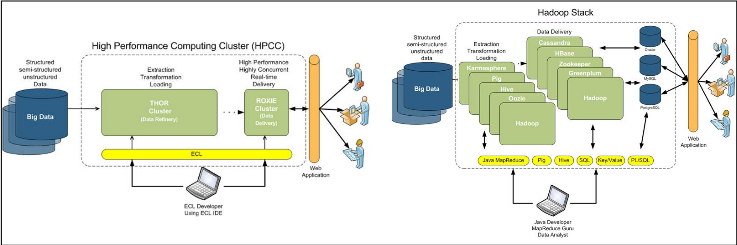
\includegraphics[width=\textwidth]{Selection_039.png}
  \caption{Comparison between HPCC System Platform and Hadoop architecture \cite{hpcc}}
  \label{hpcccomp}
\end{figure*}

\subsubsection{\textbf{Other technologies}}
There are some other type of vertically scalable technologies such as -
\begin{itemize}
\item Graphic Processing Unit (GPU)
\item Field Programmable Gate Arrays (FPGA)
\item Multicore CPUs
\end{itemize}
All of them have their own advantages and disadvantages, but all the technologies are mainly based on parallel computing.

\section{Limitations of MapReduce and Beyond}
When the Hadoop stack was first introduced, YARN was designed to overcome some of the major limitations of the MapReduce framework. Although MapReduce is a very important framework in big data analysis, there are still performance issues, reduced optimization, reduced usability, etc. We will now see some of the limitations of MapReduce framework. \cite{kalavri2013mapreduce}

\subsection{Limitations of MapReduce}
\subsubsection{Performance Issues}
MapReduce advocates of providing a highly scalable, fault-tolerant and a high performance framework. But in reality, the performance highly depends on the application and use of the framework. A quite large time of execution in Hadoop MapReduce is used in task initialization. scheduling, coordination and monitoring. Also, one big issue is that MapReduce does not employ any pipelining between Map stage and Reduce stage. This is a real performance blockage in terms of fast execution.

\subsubsection{Programming Model Issues}
MapReduce is a very elegant approach for formulating Big Data computations. But in reality, MapReduce task formulations require deep understanding of the system architecture, and what goes on behind the scenes of the computer. Even the most trivial concepts are very hard to implement in the MapReduce framework.

\subsubsection{Iterative Programming Bottleneck}
MapReduce is very inefficient when it comes to running iterative algorithms. In an iterative algorithms, Mappers read the same data again and again from the disk, and the results need to be written to the disk for further iterations. This poses a huge bottleneck with disc accesses and this degrades the performance.

\subsubsection{Configuration and Automation Issue}
Hadoop Stack (which houses the MapReduce framework) is not very easy to deploy. Each configuration option affects the performance significantly.  Proper tuning of these parameters requires knowledge of both available hardware and workload characteristics, while misconfiguration might
lead to inefficient execution and underutilization of resources.

\subsection{Beyond MapReduce}
Many solutions have come up in order to deal with the above mentioned limitations. Some are optimization methods over the existing MapReduce Framework, others are a different use of technology altogether. Some workarounds such as forward scheduling (setting up the next MapReduce job before the previous one finishes) have been proposed. However, these approaches introduce additional levels of complexity in the source code. One such work called HaLoop \cite{bu2010haloop} extends MapReduce with programming support for iterative algorithms and improves efficiency by adding caching mechanisms. CGL MapReduce \cite{ekanayake2008mapreduce}, \cite{palit2012scalable} is another optimization that focuses on improving the iterative computation performance of MapReduce. Other examples of iterative MapReduce include Twister \cite{ekanayake2010twister} and imapreduce \cite{zhang2012imapreduce}. There are also platforms such as MapReduce Online \cite{condie2010mapreduce} which solves pipelining limitations, but again making the source code quite complex. Also, there are some estimation result methods of MapReduce, where we obtain the estimated results of the computation, but overcome the performance overheads.

\section{Conclusion}
In this term paper, we have seen how Big Data can become a golden repository of information. There are many challenges for extracting information out of Big Data, but many technologies solve this concept block. We also looked how MapReduce has become a great framework for computation over Big Data. MapReduce provides a sophisticated and distributed platform and helps in making Big Data more comprehensible. Though there are limitations of MapReduce, but there are also many other solutions which would offer an alternative over the current framework depending on case-to-case and idea-to-idea. Big Data is a very vast topic of study which would require still a few years to develop in a more extensible fashion. But the concept of 3Vs of Big Data would remain the same irrespective of any technology.

\section*{Acknowledgment}

I would like to thank our faculty Dr. Arti Kashyap for guiding throughout the Term Paper.


% Can use something like this to put references on a page
% by themselves when using endfloat and the captionsoff option.
\ifCLASSOPTIONcaptionsoff
  \newpage
\fi



% trigger a \newpage just before the given reference
% number - used to balance the columns on the last page
% adjust value as needed - may need to be readjusted if
% the document is modified later
%\IEEEtriggeratref{8}
% The "triggered" command can be changed if desired:
%\IEEEtriggercmd{\enlargethispage{-5in}}

% references section

% can use a bibliography generated by BibTeX as a .bbl file
% BibTeX documentation can be easily obtained at:
% http://mirror.ctan.org/biblio/bibtex/contrib/doc/
% The IEEEtran BibTeX style support page is at:
% http://www.michaelshell.org/tex/ieeetran/bibtex/
%}
% argument is your BibTeX string definitions and bibliography database(s)
\bibliography{references}
\bibliographystyle{IEEEtran}
%
% <OR> manually copy in the resultant .bbl file
% set second argument of \begin to the number of references
% (used to reserve space for the reference number labels box)
% \begin{thebibliography}{1}

% \bibitem{bdcbook}
% H.~Kopka and P.~W. Daly, \emph{A Guide to \LaTeX}, 3rd~ed.\hskip 1em plus
%   0.5em minus 0.4em\relax Harlow, England: Addison-Wesley, 1999.

% \end{thebibliography}

% biography section
% 
% If you have an EPS/PDF photo (graphicx package needed) extra braces are
% needed around the contents of the optional argument to biography to prevent
% the LaTeX parser from getting confused when it sees the complicated
% \includegraphics command within an optional argument. (You could create
% your own custom macro containing the \includegraphics command to make things
% simpler here.)
%\begin{IEEEbiography}[{\includegraphics[width=1in,height=1.25in,clip,keepaspectratio]{mshell}}]{Michael Shell}
% or if you just want to reserve a space for a photo:
\end{document}


